\documentclass[11pt]{article}

\input{../../utils/preamble_problemas}

\title{Introducción a las matemáticas}
\author{Manuel Carlevaro}
\date{Universidad de Navarra}


\begin{document}
%\maketitle

\begin{center}
\framebox[1.0\textwidth][c]{
\huge{\textsc{Introducción a las matemáticas}} 
}
\end{center} 

\begin{center}
\vspace{1em}
\Large{\textsc{Universidad de Navarra}} 
\end{center}

 \vspace{1em}

\begin{center}
\begin{tabular}{r l}
 \textbf{Tema:} & Conjuntos numéricos. \\
 \textbf{Profesor:} & Manuel Carlevaro \\
\end{tabular}\end{center}

\vspace{2em}
\section*{Actividad 1: conjuntos, pertenencia e inclusión.}

En la siguiente actividad se repasarán las definiciones y los símbolos presentados en las secciones: definición por comprensión, definición por extensión, inclusión de conjuntos, subconjuntos, pertenencia y diagramas de Venn.

\begin{exercise}
Considerar los siguientes conjuntos y completar con $\in$ o $\notin$:
\begin{enumerate}[a)]
    \item El conjunto $A$ está formado por: perro, gato, caballo, vaca y pato. \\[1.0em]
        vaca\blank{blank}$A$, elefante\blank{}$A$, tigre\blank{}$A$, caballo\blank{}$A$, perro\blank{}$A$.
    \item El conjunto $B$ está formado por países de Europa: \\[1.0em]
        Grecia\blank{}$B$, Burkina Faso\blank{}$B$, Italia\blank{}$B$, Portugal\blank{}$B$, Brasil\blank{}$B$. 
\end{enumerate}
\end{exercise}

\begin{exercise}
El conjunto $N$ está formado por las notas musicales. Representarlo por extensión y por comprensión.
\begin{enumerate}[a)]
    \item Por extensión: \blank[width=10cm]{}
    \item Por comprensión: \blank[width=10cm]{}
\end{enumerate}
\end{exercise}

\begin{exercise}
Considerar los conjuntos $A$, $B$ y $C$ que se representan a continuación en un diagrama de Venn. 
\begin{minipage}{0.45\textwidth}
\begin{enumerate}[a)]
    \item Representar los conjuntos por extensión:\\[0.5em]
        $A$: \blank[width=4cm]{} \\[0.5em]
        $B$: \blank[width=4cm]{} \\[0.5em]
        $C$: \blank[width=4cm]{} 
    \item Completar con $\subseteq$ o $\nsubseteq$ según corresponda: \\[0.5em]
        $B$ \blank{} $A$, $C$ \blank{} $A$, $C$ \blank{} $B$.
\end{enumerate}

\end{minipage}
\hfill
\begin{minipage}{0.45\textwidth}
    \begin{center}
        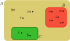
\includegraphics[width=1.0\textwidth]{figs/ej-01.pdf}
    \end{center}
\end{minipage}
\end{exercise}

\begin{exercise}
Considerar $A$, $B$ y $C$ los conjuntos definidos por comprensión de la siguiente manera:
\begin{align*}
    A &= \{\text{letras de la palabra ``vacaciones''} \} \\
    B &= \{\text{letras de la palabra ``canciones''} \} \\
    C &= \{\text{letras de la palabra ``oraciones''} \} 
\end{align*}
\begin{enumerate}[a)]
    \item Escribir por extensión los conjuntos $A$, $B$ y $C$.
    \item Decidir si se cumplen algunas de las siguientes inclusiones. En caso negativo, explicar por qué.
        \begin{multicols}{4}
        \begin{enumerate}[i)]
            \item $B \subseteq A$
            \item $B \subseteq C$
            \item $C \subseteq B$
            \item $C \subseteq A$
        \end{enumerate}
    \end{multicols}
\item Realizar un diagrama de Venn que represente los conjuntos $a$, $B$ y $C$.
\end{enumerate}
\end{exercise}

\begin{exercise}
    Escribir por comprensión al conjunto $E = \{$c, o, n, j, u, n, t$\}$. Dar tres ejemplos de subconjuntos de $E$.
\end{exercise}

\begin{exercise}
Completar con $\subseteq$ o $\nsubseteq$ según el diagrama de Venn presentado.

\begin{minipage}{0.4\textwidth}
\begin{align*}
    &A \blank{} B &B \blank{} C\\
    &C \blank{} A &C \blank{} B\\
    &B \blank{} A &B \blank{} D\\
    &D \blank{} A &C \blank{} D
\end{align*}
\end{minipage}
\hfill
\begin{minipage}{0.5\textwidth}
    \begin{center}
        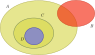
\includegraphics[width=0.9\textwidth]{figs/ej-02.pdf}
    \end{center}
\end{minipage}
\end{exercise}

\begin{exercise}
    Considerar los conjuntos $F = \{1, 2, 3, 4, 5\}$, $G = \{2, 4\}$ y $H = \{2, 4, 6\}$.
    \begin{enumerate}[a)]
        \item Decidir si las siguientes afirmaciones son verdaderas o falsas:
            \begin{multicols}{3}
                \begin{enumerate}[i)]
                    \item $2 \in F$
                    \item $4 \notin H$
                    \item $F \subseteq G$
                    \item $G \subseteq F$
                    \item $\{1, 3\} \subseteq F$
                    \item $H \nsubseteq G$
                \end{enumerate}
            \end{multicols}
        \item Realizar un diagrama de Venn que represente a los conjuntos $f$, $G$ y $H$.
    \end{enumerate}
\end{exercise}

\section*{Actividad 2: operaciones con conjuntos.}

\begin{exercise}
    Considerar los conjuntos $A = \{a, b, c, d, e\}$, $B = \{a, b, c\}$ y $C = \{d, e, f, g\}$. Calcular los siguientes conjuntos:
    \begin{multicols}{6}
        \begin{enumerate}[a)]
            \item $A \cup B$
            \item $A \cap B$
            \item $A - B$
            \item $B - A$
            \item $A \cup C$
            \item $A\cap B \cap C$
        \end{enumerate}
    \end{multicols}
\end{exercise}

\begin{exercise}
En cada caso, sombrear la región del diagrama de Venn que le corresponde a cada operación.
\begin{multicols}{3}
    \begin{enumerate}[a)]
        \item $A \cup B$ \\
            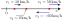
\includegraphics[scale=0.7]{figs/fig-07.pdf}
        \item $A \cap B$ \\
            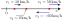
\includegraphics[scale=0.7]{figs/fig-07.pdf}
        \item $C - B$\\
            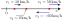
\includegraphics[scale=0.7]{figs/fig-07.pdf}
        \item $A \cup B - C$\\
            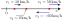
\includegraphics[scale=0.7]{figs/fig-07.pdf}
        \item $A \cup B$\\
            
\includegraphics[scale=0.7]{figs/fig-08.pdf}
        \item $A \cap B$\\
            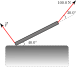
\includegraphics[scale=0.7]{figs/fig-09.pdf}
    \end{enumerate}
\end{multicols}
\end{exercise}

\begin{exercise}
Escribir la operación indicada en cada diagrama de Venn.
\begin{multicols}{2}
    \begin{enumerate}[a)]
        \item 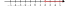
\includegraphics[scale=1.0]{figs/fig-10.pdf}
        \item 
\includegraphics[scale=1.0]{figs/fig-11.pdf}
    \end{enumerate}
\end{multicols}
\end{exercise}

\begin{exercise}
En una escuela hay 75 personas que saben tocar alguno de los siguientes instrumentos musicales: flauta, guitarra o piano. Del total de personas en la escuela hay dos personas que saben tocar los tres instrumentos. Hay 15 personas que solamente saben tocar la flauta, y hay 12 personas que solamente saben tocar el piano. También hay 9 personas que saben tocar el piano y la guitarra pero no saben tocar la flauta; dos personas que solamente saben tocar el piano y la flauta pero no saben tocar la guitarra, y dos personas que saben tocar la guitarra y la flauta pero no saben tocar el piano. ¿Cuántas personas saben tocar únicamente la guitarra?
\end{exercise}


\end{document}
